\documentclass[11pt]{article}
\usepackage{geometry} % see geometry.pdf on how to lay out the page. There's lots.
\usepackage{hyperref}
\usepackage{graphicx}
\usepackage{gensymb}
\usepackage[affil-it]{authblk}
\usepackage[toc,page]{appendix}
\usepackage{pifont}
\usepackage{amsmath}
\usepackage{amssymb}
\usepackage{relsize}
\usepackage{draftwatermark}

\SetWatermarkText{DRAFT}
\SetWatermarkScale{6}
\SetWatermarkLightness{0.95}

\DeclareMathOperator{\atantwo}{atan2}
\DeclareMathOperator{\sign}{sign}

% \geometry{letter} % or letter or a5paper or ... etc
% \geometry{landscape} % rotated page geometry

% See the ``Article customise'' template for come common customisations

\title{On Simple Planar Variable Geometry Trusses}
\author{Robert L. Read
  \thanks{read.robert@gmail.com}
}
\affil{Founder, Public Invention, an educational non-profit.}


\date{\today}

%%% BEGIN DOCUMENT
\begin{document}

\maketitle

%% \tableofcontents

\section{Introduction}

A {\em variable geometry truss} is a truss in which changes shape by means of the change of the length of members, in contrast
to many robot arms which change joint angles. We call a member which can change length an {\em actuator}.
A truss constructed purely by starting with a triangle and repeatedly adding two members and a new joint to one side of an existing triangle
to form a new triangle is a {\em simple truss}. This paper
is concerned only with simple planar trusses. In particular, we focus on trusses isomorphic to the Warren truss (e.g., an unbranching configuration of triangles.)
Furthermore, although the world {\em truss} connotes forces and structural analysis,
we are concerned purely with geometry. Although motivated by robotics, we assume that our trusses and actuators are strong enough that
we need not consider the forces acting upon the truss---in other words, we are treating it as mechanism and not a machine.

If we imagine a joint, usually at one end of our truss, to be an end effector, 
the fundamental goal of this paper is to answer the question:
\begin{quote}
  How does a change in length of an actuator change the position of an end effector?
\end{quote}

\section{Formulation}

A {\em truss} structure is a graph and a set of fixed nodes $T=(G,F)$. $G = (V,E)$. $V$ is a set of nodes or joints. $E$ is a set of lines or members which are 2-element subsets of $V$.
At least two nodes are considered to be fixed in space via a set of fixed nodes $F = {(i,x,y) \| i \in V \and x,y \in \mathbb{R}}$.

We number joints from zero and designate them with a subscript. Members are designated by two subscripts, naming the joints they connect.

A {\em configuration} is a function mapping each member of a truss structure to a non-negative length. $C: V \times V \mapsto \mathbb{R}$.

A {\em geometry} is a placement of each joint in the Cartesian plane. $G: V \mapsto \mathbb{R} \times \mathbb{R} $.

A {\em simple truss} is a truss constructed from a triangle by adding a single joint and two members to a side repetitively.
A {\em Warren truss} is an unbranched simple truss, which is isomorphic to a truss that is a single chain of equilateral triangles.
Furthermore, we insist that each even node $n$ occurs as a anti-clockwise turn (in the anti-clockwise semiplane) from the vector $\overrightarrow{n-2,n-1}$, and
each odd node occurs as a clockwise turn (in the clockwise semiplane) from the previous to nodes.

For a Warren truss, there is a simple algorithm $W$ for computing a geometry from a configuration: $W : C \mapsto G$.

A goal joint is a joint $j$ such that $j \in V$ and a desired position given by a goal function $d : V \mapsto \mathbb{R}^2$. In robotics,
a goal joint is often called an {\em end effector}.

A {\em scoring function} is a function that that takes a geometry and returns a real, non-negative value based on 
the goal node positions given by by a goal function and the actual position given by a Geometry. A score of zero is considered
 a perfect score and the a higher score represents a less sought-after result.

A {\em linear distance scoring function} is a special scoring function that that takes a geometry and returns a real, non-negative value based solely
on a summation of distances between the goal node positions given by by a goal function and the actual position given by a Geometry.

A truss {\em problem} $P = (T,d,s)$ is a truss with a scoring function and a desired position function.
A solution to a problem is a configuration and a geometry. An optimal solution is a solution which minimizes the score.

Our fundamental goal is to develop a formula for the partial derivative of the end effector
with respect to the change in length of a member.

A further goal is to be able to render a diagram illustrating the impact on the end-effector
of a change of each member, as drawn by rendering a vector from the center point of each member.

A further goal is to have algorithms to determine:
\begin{itemize}
\item What is the minimum overall change in length to a group of actuators to solve a Problem?
\item Can a Problem be solved with a single change in length?
\item Assuming bounds on the lengths of actuators, can we solve Problems?
  \item What is the workspace of a truss?
  \end{itemize}

In the remainder of this paper we will consider only Warren trusses, linear distance scoring functions, and desired position functions
that map only one node, called an end effector, to a desired position. Furthermore, we will assume that the first two nodes are fixed
and that the furthest node (by path length) from the first node is the end effector.

\section{Moving an External Member}

We seek a formula for the change in position of the end effector $e$ with respect to change in the length of a member given a geometry.
In the case of a Warren truss, all members can be divided between external members and internal members. A change to the length of an
external member is particularly simple.

The change in position is a centered on the goal node representing the place the goal node would move to with a unit change in length.
However, the derivative is only valid as an infinitessimal, but as an infinitessimal its magnitude and direction may be usefully
added to or compared to other such vectors. We can thus usefully tell which member would change the position of the goal node most
rapidly in response to a minute change in different members.

\begin{figure}
  \centering
  \includegraphics[width=\textwidth]{External_angle_Change.png}
  \caption{A Trusss Problem with Change to an External Member Length}  
\end{figure}

The fundamental observation is that for an external member $(C,A)$, a change in length generates a rotation $\theta$ about joint $B$
whose position is given by $(B_x,B_y)$. $\theta$ is the angle of the vector from the pivot point $B$ to the end-effector $E$ with the $x$-axis.
This rotation applies to the triangle defined by three joints: $\triangle B,C,E$. Not that this triangle doeS not exist as a physical
structure in the truss. 

By using the law of cosines, where $a = \|\overrightarrow{A,B}\|, b = \|\overrightarrow{A,C}\|, c = \|\overrightarrow{B,C}\| $,
where $b$ is the member opposite the pivot joint $B$ which changes the angle $ \phi_{i-1} = \angle ABC $. In other words, $\phi$ is a signed angle measure
$BA$ moved into $BC$, with positive representing anti-clockwise.
\[
\cos{\phi} = \frac{a^2 - b^2 + c^2}{2 a c}
\]
or
\[
\phi = \arccos{\frac{a^2 - b^2 + c^2}{2 a c}}
\]
Using Woflram Alpha to differentiate this, we obtain:

\[
\frac{\partial \phi}{\partial b} = \frac{b}{ac\sqrt{1 - \frac{(a^2 + c^2 - b^2)^2}{4a^2c^2}}}
\]

This derivation loses the sign information, which we recover by considering whether $S = \sign{\phi}$.

The change in the end effector is always perpendicular to the drawn from the pivot joint to the effector and proportional to its length.
An alternative way of looking at this is that the result should be orthogonal to the vector
\[
\begin{bmatrix}
           (e_x  - x) \\
           (e_y - y)  \\
\end{bmatrix}
\]
In other words:
\[
S \cdot
\begin{bmatrix}
           - (e_y  - y) \\
           (e_x - x)  \\
\end{bmatrix}
\]
With the sign $S$ is negative if $\phi$ is clockwise. $\phi$ cannot be zero or equal or exceed $\pi$ in a physical machine is excluded for that reason.

Since the change in $\phi$ is equal to the change in $\theta$, we can use the chain rule:

\[
\frac{\partial e}{\partial  b} = \begin{bmatrix}
           \frac{\partial e_x}{\partial b} \\
           \frac{\partial e_y}{\partial b} \\
         \end{bmatrix} = \frac{Sb}{ac\sqrt{1 - \frac{(a^2 + c^2 - b^2)^2}{4a^2c^2}}} \begin{bmatrix}
           -(e_y -y)  \\
           (e_x - x )  \\
         \end{bmatrix}
\]

So this is a closed-form expression for the change in the position of an end effector for any external member $i,i-2$ we choose. If we then know how the
scoring functions changes as the end effector moves, we can compute the change in the scoring functions as we change $b = \| AC \|$, which is what
we need for numeric optimization.

\section{Moving an Internal Member}


In the Internal Member Length change diagram, $\angle ABC = \beta $, $\angle CBD = \psi$, $\angle BCD = \chi$,
$\angle ACB = \gamma$, $\angle ADC \delta$, and $\angle BAC = \alpha$. The lengths are marked $a,b,c,f,g$, with $a$ being opposite node $A$ and a diagonal
of the quadrilateral $ABDC$.




Furthermore, $\angle ABD = \beta + \psi$, and $\angle ACD = \gamma + \chi$.

The absolute angle between the line between the fixed nodes $A$ and $B$ and the $x$-axis is $\rho$ (counting positive as anticlockwise from the $x$-axis.)
Both $A$ and $B$ are considered fixed, but both $C$ and $D$ move as $a$ changes. $D$ rotates about $B$ and $C$ rotatest about $A$.

\begin{figure}
  \centering
  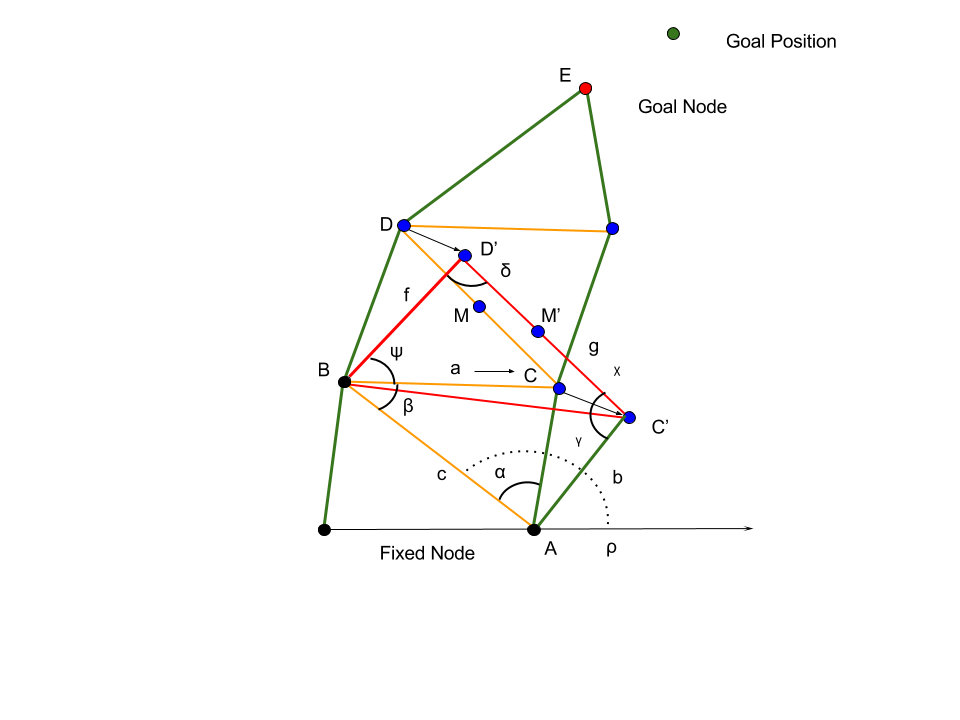
\includegraphics[width=0.7\textwidth]{Internal_angle_change.png}
  \caption{A Trusss Problem with Change to an Internal Member Length}  
\end{figure}


Because the member $DC$ does not change its length, we conceptualize the impact of a change to length $a$ as translating  between $C$ and $D$ and
rotating $BC$ about $M$. By knowing the change in the absolute rotation and the change in the position of $M$ as $a$ changes infintessimally, we know how the
end effector $E$ changes.


We can compute $\frac{\partial \beta}{\partial a}$ directly (using Wolfram Alpha) from $\phi$:
\[
\beta = \arccos{\frac{a^2 - b^2 + c^2}{2 a c}}
\]

\[
\frac{\partial \beta}{\partial a} =
-\frac{\frac{1}{c} - \frac{a^2 - b^2 + c^2}{2 a^2 c}}
{\sqrt{1 - \frac{(a^2 - b^2 + c^2)^2}{4 a^2 c^2}}}
\]

Calculating the same way for $\alpha$ in order to have $C$
\[
\alpha = \arccos{\frac{-a^2 +  b^2 + c^2}{2 b c}}
\]

\[
\frac{\partial \alpha}{\partial a} =
\frac{a}
{bc \sqrt{1 - \frac{(-a^2 + b^2 + c^2)^2}{4 b^2 c^2}}}
\]

\[ \gamma = \pi - (\alpha + \beta) \]

Now we compute $\chi$ from the law of cosines:
\[
\chi = \arccos{\frac{a^2 - f^2 + g^2}{2 a g}}
\]

\[
\frac{\partial \chi}{\partial a} =
-\frac{\frac{1}{g} - \frac{a^2 - f^2 + g^2}{2 a^2 g}}
{\sqrt{1 - \frac{(a^2 - f^2 + g^2)^2}{4 a^2 g^2}}}
\]


\[
\begin{bmatrix}
  C_x \\
  C_y \\
\end{bmatrix} =
\begin{bmatrix}
 A_x + b \cos{(\rho - \alpha)} \\
 A_y + b \sin{(\rho - \alpha)} \\
\end{bmatrix}
\]

Taking the derivative of this with respect to $a$,

\[
\begin{bmatrix}
  \frac{\partial C_x}{\partial a} \\
  \frac{\partial C_y}{\partial a} \\
\end{bmatrix} =
\begin{bmatrix}
 0 + \frac{\partial b \cos{(\rho - \alpha)}}{\partial a} \\
 0 + \frac{\partial b \sin{(\rho - \alpha)}}{\partial a} \\
\end{bmatrix} =
\begin{bmatrix}
b \frac{a\sin{(\rho - \alpha)}}
{bc \sqrt{1 - \frac{(-a^2 + b^2 + c^2)^2}{4 b^2 c^2}}}
  \\
- b \frac{a\cos{(\rho - \alpha)}}
{bc \sqrt{1 - \frac{(-a^2 + b^2 + c^2)^2}{4 b^2 c^2}}}
  \\
\end{bmatrix} =
\frac{a}{c \sqrt{1 - \frac{(-a^2 + b^2 + c^2)^2}{4 b^2 c^2}}}
\begin{bmatrix}
 \sin{(\rho - \alpha)}  \\
- \cos{(\rho - \alpha)}  \\
\end{bmatrix}
\]


The angle $\theta$ between $CD$ and the $x$-axis is therefore given by:
\begin{align*}
  \theta &= \\
  (\rho - \alpha) + (\pi - (\chi + \gamma)) &= \\
\rho + \pi - (\alpha + \chi + (\pi - (\alpha + \beta)) &= \\
\rho + \pi - (\chi + (\pi  -\beta))  &= \\
\rho + -\chi + \beta
\end{align*}
We seek $\frac{\partial \theta}{\partial a}$.

\[
\frac{\partial \theta}{\partial a} = 0 - \frac{\partial \chi}{\partial a} +
\frac{\partial \beta}{\partial a} =
\frac{\frac{1}{c} - \frac{a^2 - b^2 + c^2}{2 a^2 c}}
{\sqrt{1 - \frac{(a^2 - b^2 + c^2)^2}{4 a^2 c^2}}}
-\frac{\frac{1}{g} - \frac{a^2 - f^2 + g^2}{2 a^2 g}}
{\sqrt{1 - \frac{(a^2 - f^2 + g^2)^2}{4 a^2 g^2}}}
\]

Now $E$ is simply a translation by $\frac{\partial C}{\partial a}$ by a rotation
about $C$, which as we have previously shown

\[
\frac{\partial e}{\partial  a} = 
\begin{bmatrix}
  \frac{\partial C_x}{\partial a}  \\
  \frac{\partial C_y}{\partial a} \\
  \end{bmatrix}
 +
(\frac{\frac{1}{c} - \frac{a^2 - b^2 + c^2}{2 a^2 c}}
{\sqrt{1 - \frac{(a^2 - b^2 + c^2)^2}{4 a^2 c^2}}}
-\frac{\frac{1}{g} - \frac{a^2 - f^2 + g^2}{2 a^2 g}}
{\sqrt{1 - \frac{(a^2 - f^2 + g^2)^2}{4 a^2 g^2}}})
\begin{bmatrix}
           -(e_y -C_y)  \\
           (e_x - C_x )  \\
         \end{bmatrix}
\]

\[
\frac{\partial e}{\partial  a} =
\frac{a}{c \sqrt{1 - \frac{(-a^2 + b^2 + c^2)^2}{4 b^2 c^2}}}
\begin{bmatrix}
 \sin{(\rho - \alpha)}  \\
- \cos{(\rho - \alpha)}  \\
\end{bmatrix}
 +
\Bigg(\frac{\frac{1}{c} - \frac{a^2 - b^2 + c^2}{2 a^2 c}}
{\sqrt{1 - \frac{(a^2 - b^2 + c^2)^2}{4 a^2 c^2}}}
-\frac{\frac{1}{g} - \frac{a^2 - f^2 + g^2}{2 a^2 g}}
{\sqrt{1 - \frac{(a^2 - f^2 + g^2)^2}{4 a^2 g^2}}}
\Bigg)
\begin{bmatrix}
           -(e_y -C_y)  \\
           (e_x - C_x )  \\
         \end{bmatrix}
\]


In computing all of this, one must be very careful to keep the signs straight.








\section{Testing}

The best way to test this is to build a diagram that draws the vector $\frac{\partial e}{\partial l_{BC}}$ at at the center
of each edge $\vec{BC}$. This should allow both the direction and magnintude to be visualized in a reasonable way.
We could call this a {\em delta diagram}.

  


\section{References}



\end{document}

http://eprints.cs.vt.edu/archive/00000192/01/TR-90-10.pdf


https://people.eecs.berkeley.edu/~elghaoui/Teaching/EE227A/lecture6.pdf

http://homes.cs.washington.edu/~sagarwal/aat.pdf

http://zoonek.free.fr/blosxom/R/2012-06-01_Optimization.html

http://docs.mosek.com/modeling-cookbook/cqo.html

// This one looks pretty interesting
http://ieeexplore.ieee.org/abstract/document/4160811/

https://tspace.library.utoronto.ca/bitstream/1807/14046/1/NQ49815.pdf



\section{Moving an Internal Member}

Note: I believe the expression for the moving the node is as simple as $\frac{d\rho}{dz} = \frac{1}{\cos{\alpha} L}$, where $\alpha$ is the angle between the rods, and $\rho$ $z$ is the length
of the changed rod, and $L$ is the length of the moved node $\vec{AC}$. We can then solve for the interior triangle comletely. The final action can be thought of as
a translation of either $D$ or $C$ and a rotation about that point. This computation will end up using absolute angles (relative to the axes) in it compuation.)

Moving an internal member is slightly more complicated. In a Warren Truss, moving an internal member is in fact
changing the shape of a parallelogram.  The best way to think of the overall transformation of an end effector is
to imagine it as both a translation and a rotation of the midpoint of one of the edges of the parallelogram.

We need to develop the formulae for the derivatives of the motions of both endpoints and add them together to obtain this.
The motion of each point, however, is a pure translation.

Given that we are dealing with infinitessimal motion, the partial derivative of $C$ is easy
because it must be at right angles to $\vec{AC}$. Let $\rho$ be the anticlockwise angle $AC$ makes with the $x$-axis.

\[
\frac{\partial C}{\partial  l_{BC}} = \begin{bmatrix}
           \frac{\partial C_x}{\partial l_{BC}} \\
           \frac{\partial C_y}{\partial l_{BC}} \\
         \end{bmatrix} = \begin{bmatrix}
           \sin{\rho}  \\
           \cos{\rho} \\
         \end{bmatrix}
\]

To find the partial derivative of the $D$'s motion, we utlize the fact that the lengths of $\vec{BD}$ and $\vec{CD}$ don't change.
We thus have three lengths and two points, from which the third point ($D$) can be computed. The easily way to do this
is to assume that the point $B$ is at the origin, and compute the angle of $\vec{BD'}$. This is the sum of the angle $\angle D'BC'$
which can be obtained from the law of cosines, and the angle of $\vec{BC'}$ with the $x$ axis.

\[
\angle D'BC' = \arccos{\frac{c^2 + d^2 - b^2}{2cd}}
\]

\[
\angle \vec{BC'} = \atantwo( C'_y - B_y ,  C'_x - B_x )
\]

\[
\psi = \angle \vec{BD'} = \angle D'BC' + \angle \vec{BC'}
\]

\[
\psi = (\arccos{\frac{c^2 + d^2 - b^2}{2cd}} +  \atantwo( C'_y - B _y,  C'_x - B_x))
\]

\[
D' = \delta \cdot \begin{bmatrix}
          \sin{ \angle \vec{BD'} } \\
          \cos{ \angle \vec{BD'} } \\
\end{bmatrix} +
\begin{bmatrix}
           B_x  \\
           B_y \\
\end{bmatrix} =
\delta \cdot 
\begin{bmatrix}
          \sin{ \psi } \\
          \cos{ \psi } \\
\end{bmatrix} +
\begin{bmatrix}
           B_x  \\
           B_y \\
         \end{bmatrix}
\]

\[
D' =
\delta \cdot 
\begin{bmatrix}
          \sin{ \psi } \\
          \cos{ \psi } \\
\end{bmatrix} +
\begin{bmatrix}
           B_x  \\
           B_y \\
         \end{bmatrix}
\]

Given that $\delta$ is the differential change in length, this can be rewritten as derivative:

\[
\frac{\partial D}{\partial  l_{BC}} = \begin{bmatrix}
           \frac{\partial D_x}{\partial l_{BC}} \\
           \frac{\partial D_y}{\partial l_{BC}} \\
         \end{bmatrix} = \begin{bmatrix}
           \sin{\psi}  \\
           \cos{\psi} \\
\end{bmatrix}
\]



Now to understand how a change to the $\vec{BC}$ length effects the end effector, we can
add the partial derivatives of $C$ and $D$ in order to get the translational change
to the midpoint $P$ of $\vec{CD}$. Then separately we must compute the change in the angle
of the vector $\vec{CD}$. These things together will allow us to compute the
partial derivative of the end effector $e$.

\[
\frac{\partial P}{\partial  l_{BC}} =
\frac{\partial C}{\partial  l_{BC}} = \begin{bmatrix}
           \frac{\partial C_x}{\partial l_{BC}} \\
           \frac{\partial C_y}{\partial l_{BC}} \\
         \end{bmatrix} \begin{bmatrix}
           \frac{\partial D_x}{\partial l_{BC}} \\
           \frac{\partial D_y}{\partial l_{BC}} \\
\end{bmatrix}
= \begin{bmatrix}
           \sin{\rho}  \\
           \cos{\rho} \\
         \end{bmatrix}
 +
 \begin{bmatrix}
           \sin{\psi}  \\
           \cos{\psi} \\
\end{bmatrix}
 \]

 Moving the member $\vec{BC}$ in general induces a rotation about $P$ as well.

 \[
 \rho = \angle{\vec{CD}} - \angle{\vec{C'D'}}
 \]

 \[
 \rho = \angle{\atantwo{D'_y - C'_y}{D'_x - C'_x}}
 \]

 Since:

 \[
 \frac{d}{dx} \atantwo{g(x)}{f(x)} = \frac{g(x)f'(x) - f(x)g'(x)}{f(x)^2 + g(x)^2}
 \]
 , we have:

 
 
\[
\frac{\partial \rho}{ \partial l_{BC}} = \frac{ (D'_x - C'_x)\frac{\partial (D'_y - C'_y)}{\partial l_{BC}}
  - (D'_y - C'_y)\frac{\partial (D'_x - C'_x)}{\partial l_{BC}}
}
  {(D'_y - C'_y)^2 + (D'_x - C'_x)^2}
  \]

  I always get confused between differentials and derivatives.  However, if we evaulate this instantaneously,
  we can replace $D'$ with $D$ and $C'$ with $C$. We already have closed form expressions for the other partials.

  \[
\frac{\partial \rho}{ \partial l_{BC}} = \frac{ (D'_x - C'_x)\frac{\partial (D'_y - C'_y)}{\partial l_{BC}}
  - (D'_y - C'_y)\frac{\partial (D'_x - C'_x)}{\partial l_{BC}}
}
  {(D'_y - C'_y)^2 + (D'_x - C'_x)^2}
  \]

  So we have:
  
    \[
    \frac{\partial \rho}{ \partial l_{BC}} = \frac{ (D_x - C_x)(\sin{\psi} -\sin{\rho})
      - (D_y - C_y)(\cos{\psi} - \cos{\rho})}
  {(D_y - C_y)^2 + (D_x - C_x)^2}
  \]

  The change to the end effector is the composition of the translation of the midpoint and
  the rotaion about the midpoint by this angle.

  Now we can apply our basic rotation about a point formula:

  
\[
\frac{\partial e}{\partial \theta} = \begin{bmatrix}
           \frac{\partial e_x}{\partial \theta} \\
           \frac{\partial e_y}{\partial \theta} \\
         \end{bmatrix} = \begin{bmatrix}
           -(e_x  - x) \sin{\theta} + -(e_y -y)\cos{\theta}  \\
           (e_x - x ) \cos{\theta} + -(e_y - y)\sin{\theta}  \\
         \end{bmatrix}
\]

where $x,y$ is the point of rotation. In this case, we simply add the contributions due to the rotation
and the translation.

\begin{equation} \label{eq1}
\begin{split}
\frac{\partial e}{\partial l_{BC}} = 
\frac{\partial e}{\partial \rho} \frac{\partial \rho}{ \partial l_{BC}} = & \\
 & \frac{ (D_x - C_x)(\sin{\psi} -\sin{\rho})
      - (D_y - C_y)(\cos{\psi} - \cos{\rho})}
  {(D_y - C_y)^2 + (D_x - C_x)^2} \cdot \\
\begin{bmatrix}
           -(e_x  - P_x) \sin{\rho} + -(e_y - P_y)\cos{\rho}  \\
           (e_x - P_x ) \cos{\rho} + -(e_y - P_y)\sin{\rho}  \\
         \end{bmatrix}
\end{split}
\end{equation}

